\documentclass[a4paper, 10pt]{article}
\usepackage[english]{babel}
\usepackage{amsmath}
\usepackage{amsfonts}
\usepackage{amssymb}
\usepackage[font=scriptsize]{caption}
\usepackage{parskip}
\usepackage[a4paper, margin=1in, top=1.2in, columnsep=0.6cm]{geometry}
\usepackage{titling}
\usepackage{subcaption}
\usepackage{float}
\usepackage{placeins}
\usepackage{graphicx}
\usepackage{booktabs}
\usepackage{newtxtext, newtxmath}
\usepackage{enumitem}
\usepackage{siunitx}

\newcommand{\kHz}{\si{\kilo\hertz}}
\newcommand{\mH}{\si{\milli\henry}}
\newcommand{\nF}{\si{\nano\farad}}
\newcommand{\uF}{\si{\micro\farad}}
\newcommand{\V}{\si{\volt}}
\newcommand{\F}{\si{\farad}}
\newcommand{\Ohm}{\si{\ohm}}

\setlength{\parskip}{5pt plus 1pt minus 1pt}
\setlength{\droptitle}{-2cm}


\usepackage[backend=biber, style=numeric]{biblatex}
\addbibresource{references.bib}

\title{%
  \large\textbf{Electronics Laboratory: Synthesis Report}\\[4pt]
  \normalsize Experiments: Resonance, Transients, and\\
  Semiconductor Devices in AC Circuits
}
\author{
Guilherme C. Schewtschik (3748052)\\
Yaman Ajaj (3722952)
}
\date{2025}

\begin{document}
\maketitle

\begin{abstract}
\noindent
This report consolidates six electronics laboratory experiments (E12, E11e,
E13He, E14e, E17e) investigating linear and nonlinear circuit elements under
AC and transient excitation. Topics span series and parallel RLC resonance,
phase shift in reactive circuits, RC discharge transients via MOSFET
switching, semiconductor diode characteristics, and coupled LC-oscillator
normal modes. Across all experiments, model parameters such as $f_0$, $Q$,
$\tau$, $E_g$, and the coupling coefficients $k$ were extracted via
nonlinear least-squares fitting in Python and compared against values
computed directly from component specifications. We summarise the
methodology and key results for each experiment, and we identify several
inconsistencies between fitted and theoretical values that merit further
discussion.
\end{abstract}

% ─────────────────────────────────────────────────────────────────────────────
\section{Introduction}
% ─────────────────────────────────────────────────────────────────────────────

This report covers a sequence of experiments exploring the behaviour of
linear and nonlinear circuit elements, namely resistors, capacitors,
inductors, and diodes, under both AC steady-state and transient excitation.
Although the experiments address distinct physical phenomena, they share a
common methodology: a physical model is derived from circuit theory, a
measurement is performed with an oscilloscope or source-measure unit, and
the model parameters are extracted by nonlinear least-squares fitting using
\texttt{scipy.optimize.curve\_fit}.

The unifying theoretical thread is the response of $R$, $L$, $C$ networks to
sinusoidal and step excitations:
\begin{itemize}[itemsep=2pt]
  \item \textbf{Resonance} (E12): the frequency-dependent amplitude response
        of series and parallel RLC circuits, characterised by the resonance
        frequency $f_0 = 1/(2\pi\sqrt{LC})$ and quality factor $Q$.
  \item \textbf{Phase shift} (E11e): the frequency-dependent phase angle
        $\varphi(\omega)$ between current and voltage in RC, RL, and RLC
        circuits.
  \item \textbf{Transients} (E13He): the exponential charge and discharge
        response $V(t) = V_0 e^{-t/RC}$ of a capacitor switched by a MOSFET.
  \item \textbf{Nonlinear devices} (E14e): the exponential $I$--$V$
        characteristic of semiconductor diodes and the voltage dependence of
        junction capacitance.
  \item \textbf{Normal modes} (E17e): the splitting of a single resonance
        into symmetric and antisymmetric eigenfrequencies when two LC
        circuits are coupled capacitively or inductively.
\end{itemize}

Each of the following sections presents the experimental method, the key
results as reported, and a brief critical assessment comparing fitted
values against theoretical expectations from component nominal values.

% ─────────────────────────────────────────────────────────────────────────────
\section{E12: RLC Resonant Circuits}
% ─────────────────────────────────────────────────────────────────────────────

\subsection{Method}

The frequency-dependent voltage $U_R(f)$ across a damping resistor $R_d$ was
recorded for a series RLC circuit ($L = 1.5\,\mH$) at two damping
resistances, $R_d = 220\,\Omega$ and $R_d = 10\,\Omega$, over a window
$f \in [1.6, 9.0]\,\kHz$ chosen to bracket the resonance such that
$0.2 \le U_R(f)/U_R(f_0) \le 1$. A Gaussian model was fitted to each curve to
extract $f_0$ and the linewidth $\sigma$. A parallel resonant circuit,
consisting of a coil and capacitor in parallel and in series with
$R_d = 220\,\Omega$, was measured separately. Its impedance was derived
analytically before fitting a four-parameter model $I(f; L, C, R_{Sp}, R_d)$
directly to the current data.

\subsection{Results}

\begin{table}[H]
\centering
\caption{Series resonance fit results (E12, Task 2).}
\begin{tabular}{lccc}
\toprule
$R_d$ & $\Delta f$ (FWHM) & $Q = f_0/\Delta f$ & $\delta = \pi\,\Delta f$ \\
\midrule
$220\,\Omega$ & 22.5 kHz & 0.3 & 70655 \\
$10\,\Omega$  & 29.0 kHz & 0.2 & 91127 \\
\bottomrule
\end{tabular}
\end{table}

From the averaged fitted $f_0 \approx 6.82\,\kHz$ and Thomson's
relation $C = 1/[L(2\pi f_0)^2]$, the capacitance was determined as
$C = 362.6\,\nF$.

For the parallel circuit, the bounded four-parameter fit converged to
$L_{\text{fit}} = 10.0\,\mH$, $C_{\text{fit}} = 111.2\,\nF$,
$R_{Sp} = 0.1\,\Omega$, and $R_d = 10.0\,\Omega$, giving
$f_{0,\text{parallel}} = 4.77\,\kHz$, compared with
$f_{0,\text{series}} = 6.82\,\kHz$.

\subsection{Assessment}

The quality factors obtained from the FWHM fit, $Q \approx 0.2$ to $0.3$,
are inconsistent with circuit theory for one of the two resistances tested.
Using the fitted capacitance together with the nominal $L$ and $R$ values,
the theoretical quality factor of a series RLC circuit is
$Q = \frac{1}{R}\sqrt{L/C}$, which gives $Q \approx 0.29$ for
$R_d = 220\,\Omega$, matching the fit well, but $Q \approx 6.4$ for
$R_d = 10\,\Omega$. This is a sharply underdamped resonance rather than the
heavily overdamped one that was reported. Figure~\ref{fig:e12_series} shows
that both measured curves are nearly flat across the $1.6$ to
$9.0\,\kHz$ window rather than exhibiting a clear peak, which suggests
that the frequency window did not fully capture the true resonance shape
for the low-resistance case, biasing the Gaussian fit toward an
artificially broad linewidth. It is also worth noting that the reported
damping constant $\delta = \pi \Delta f$ does not correspond to the
standard definition $\delta = R/(2L)$ used in the course references
(\cite{tipler}, \cite{demtroeder}). The two only coincide under specific conventions for
$\Delta f$, and this point should be clarified in a revision.

The parallel-circuit fitted inductance of $10\,\mH$ differs by a
factor of roughly $6.7$ from the series-circuit nominal inductance of
$1.5\,\mH$, and the two resonance frequencies disagree by 30\%. Since
the same physical coil should appear in both circuits, This discrepancy suggests that the fitted model is insufficiently
constrained by the available data. The optimisation may therefore
have converged to a parameter set that reproduces the measured
response while remaining physically unrealistic. Tighter
initial guesses and bounds derived from the series-circuit results would
likely improve convergence.

\begin{figure}[H]
  \centering
  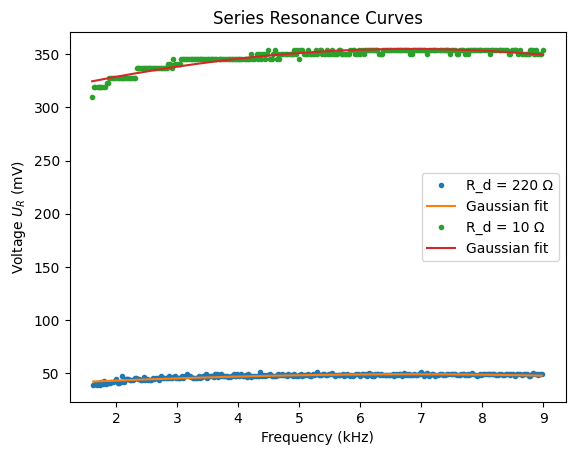
\includegraphics[width=0.45\linewidth]{../E12/series_resonance_curve.png}
  \caption{Series resonance curves for $R_d = 220\,\Omega$ and
         $R_d = 10\,\Omega$ with Gaussian fits. The broad fitted linewidth
         for the $10\,\Omega$ case contributes to the unrealistically small
         extracted quality factor.}
  \label{fig:e12_series}
\end{figure}

\newpage

% ─────────────────────────────────────────────────────────────────────────────
\section{E11e: Phase Shift in AC Circuits}
% ─────────────────────────────────────────────────────────────────────────────

\subsection{Method}

The phase shift $\varphi$ between the resistor voltage, which is in phase
with the current, and the source voltage was measured for RC, RL, and RLC
series circuits. This was done by recording the time delay $\Delta t$
between the two signals on a two-channel oscilloscope as a function of
drive frequency $f$, then converting via $\varphi = \omega\,\Delta t$ with
$\omega = 2\pi f$. The theoretical phase relations are:
\begin{equation}
  \varphi_{RC} = -\arctan\!\left(\frac{1}{\omega RC}\right), \quad
  \varphi_{RL} = \arctan\!\left(\frac{\omega L}{R}\right), \quad
  \varphi_{RLC} = \arctan\!\left(\frac{\omega L - 1/\omega C}{R}\right).
  \label{eq:phase_relations}
\end{equation}

\subsection{Results}

The RC series resistance, extracted from $R = 1/(\omega C \tan|\varphi|)$
and averaged over all frequencies, gave $R_{RC} = 330.2\,\Omega$ against a
nominal value of $R_r = 328.8\,\Omega$, a 0.44\% error. The RLC resonance
frequency was determined two ways: directly from the measured zero-crossing,
giving $f_0 = 2.68\,\kHz$, and from a linear fit to $\varphi(f)$ near
resonance extrapolated to $\varphi = 0$, giving $f_0 = 2.673\,\kHz$, a
difference of $-0.25\%$. The corresponding inductance from Thomson's
relation was $L = 6.751\,\mH$ versus a nominal value of
$6.77\,\mH$, a $-0.29\%$ error. The same inductance, extracted
independently from the RL phase relation, gave $L_{RL} = 5.633\,\mH$,
a $-16.8\%$ deviation from the nominal value.

\subsection{Assessment}

The RC resistance and the RLC-derived inductance both agree with nominal
component values to better than 0.5\%, demonstrating that the
resonance-based extraction method, which fits $\varphi(f)$ near the
zero-crossing, is robust. The RL-circuit estimate of $L$, by contrast,
shows a substantially larger error of $-16.8\%$. Since
$\varphi_{RL} = \arctan(\omega L/R)$ is a smooth, monotonic function with no
resonance feature to anchor the fit, this estimate is more sensitive to
systematic errors in the nominal resistance $R_r$ used in the formula and
to phase-measurement uncertainty at the sampled frequencies. An independent
measurement of $R_r$, for example with a multimeter, used in place of the
nominal printed value could help resolve this gap.

\begin{figure}[H]
  \centering
  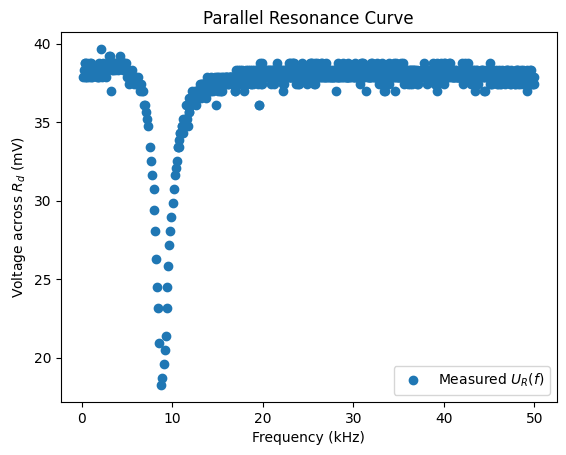
\includegraphics[width=0.45\linewidth]{../E12/parallel.png}
  \caption{Measured phase shift $\varphi(f)$ for RLC, RL, and RC series
           circuits (reproduced from the original notebook).}
  \label{fig:e11e_phase}
\end{figure}

% ─────────────────────────────────────────────────────────────────────────────
\section{E13He: Capacitor Discharge with MOSFET Switching}
% ─────────────────────────────────────────────────────────────────────────────

\subsection{Method}

An Arduino-controlled IRF520 MOSFET periodically discharged a capacitor
through a resistive path, and the voltage decay $V(t) = V_0 e^{-t/RC}$ was
recorded with a PicoScope in single-trigger, falling-edge mode. Measurements
were taken for capacitances of $1\,\nF$ and $220\,\nF$, each
through nominal discharge resistances of $1\,\text{k}\Omega$, $100\,\Omega$,
$22\,\text{k}\Omega$, and $100\,\text{G}\Omega$, the last of which is
effectively an open circuit and was included as a high-resistance control.
A two-parameter exponential $V(t) = A e^{bt}$ was fitted to a short window
around each discharge event.

\subsection{Results}

All five measurements show qualitatively similar fitted decay constants,
with $b$ ranging from $-16.9$ to $-15.9\,\mu\text{s}^{-1}$, despite spanning
more than eight orders of magnitude in nominal resistance. The fitted
curves systematically overshoot the data at early times and fail to capture
the pronounced oscillatory ringing visible immediately after the switching
edge, as shown in Figures~\ref{fig:e13_fit1} and~\ref{fig:e13_fit2}.

\subsection{Assessment}

The near-identical decay constants across four very different nominal
resistances are the clearest indicator that the measured transient is not
dominated by the intended discharge resistor. Given the
nanosecond-to-microsecond timescale of the ringing and its presence even in
the $100\,\text{G}\Omega$ open-circuit control, the observed signal is most
plausibly dominated by parasitic inductance and capacitance in the
breadboard wiring, together with the MOSFET's own switching transient,
rather than by the intended $RC$ decay. This interpretation is consistent
with the simple exponential model systematically failing to capture the
damped oscillation seen in every panel: a single real pole
$V_0 e^{-t/RC}$ cannot reproduce ringing, which requires at least a
complex-conjugate pole pair, that is, an effective series $RLC$ response
arising from stray inductance. A revised analysis should either fit a
damped sinusoid $V_0 e^{-t/\tau}\cos(\omega t + \phi)$ to this ringing
region, or select a later time window in which the parasitic oscillation
has decayed and the genuine $RC$ tail dominates.

Another possible contribution is the finite bandwidth and probe
loading of the measurement setup, which may distort very fast
transients on the nanosecond timescale.

\begin{figure}[H]
  \centering
  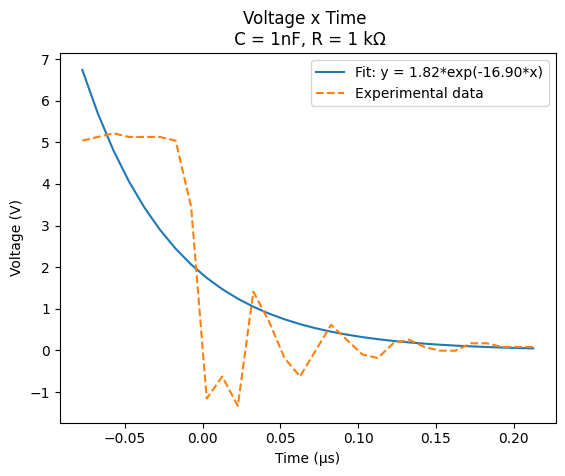
\includegraphics[width=0.45\linewidth]{../E13/Voltage_time_fit.png}
  \caption{Exponential fit versus measured discharge, $C=1\,\nF$,
         nominal $R=1\,\text{k}\Omega$. The fit reproduces the overall decay
         trend but fails to capture the oscillatory transient immediately
         after switching.}
  \label{fig:e13_fit1}
\end{figure}


% ─────────────────────────────────────────────────────────────────────────────
\section{E14e: Semiconductor Diodes}
% ─────────────────────────────────────────────────────────────────────────────

\subsection{Method}

Current-voltage characteristics were recorded for a silicon diode, an LED,
and two Zener diodes under forward and reverse bias. The Shockley diode
equation
\begin{equation}
  I = I_0\left(e^{qU/nk_BT} - 1\right)
  \label{eq:shockley}
\end{equation}
describes the forward-bias exponential rise. For the LED, the forward
threshold voltage $U_{\text{on}}$ was used to estimate the bandgap energy
via $E_g \approx qU_{\text{on}}$. Separately, the depletion-layer
capacitance $C$ was measured as a function of reverse bias $U$ with an LCR
meter, and a linear fit of $1/C^2$ versus $U$ was performed to test the
abrupt-junction relation $1/C^2 \propto U$.

\newpage

\subsection{Results}

Forward threshold voltages were approximately $0.7\,\V$ for the
silicon diode and between $2.6$ and $3.1\,\V$ for the LED, giving an
estimated bandgap of $E_g \approx 3.0\,\text{eV}$, consistent with a
blue or violet LED. Zener breakdown was observed near $5.6\,\V$ for
Zener~1 and near $0.8\,\V$ for Zener~2. The $1/C^2$ versus $U$ linear
fit gave a slope of $-1.857 \times 10^{19}\,\F^{-2}\V^{-1}$, an
intercept of $6.825\times10^{20}\,\F^{-2}$, and $R^2 = 0.70$.

\subsection{Assessment}

The forward-bias and bandgap results are physically reasonable and
internally consistent. The depletion-capacitance fit appears inconsistent with the
simplest abrupt-junction model because the fitted slope is
negative whereas a positive slope is expected theoretically.
$1/C^2 = \frac{2}{q\varepsilon N_A}(U_{bi} + U)$ predicts that $1/C^2$
increases with reverse voltage $U$, since the capacitance decreases as the
depletion width grows, meaning the slope should be positive. The fitted
slope is instead negative, and the moderate $R^2 = 0.70$ further suggests
that the data does not follow the expected linear form well over the
measured voltage range. This may indicate that the measurement was taken
predominantly in a regime where $U \ll U_{bi}$, where a more general
graded-junction capacitance model applies rather than the abrupt-junction
form, or that the voltage polarity was inverted in the dataset. This point
should be re-examined before the doping concentration is extracted from the
slope.

\begin{figure}[H]
  \centering
  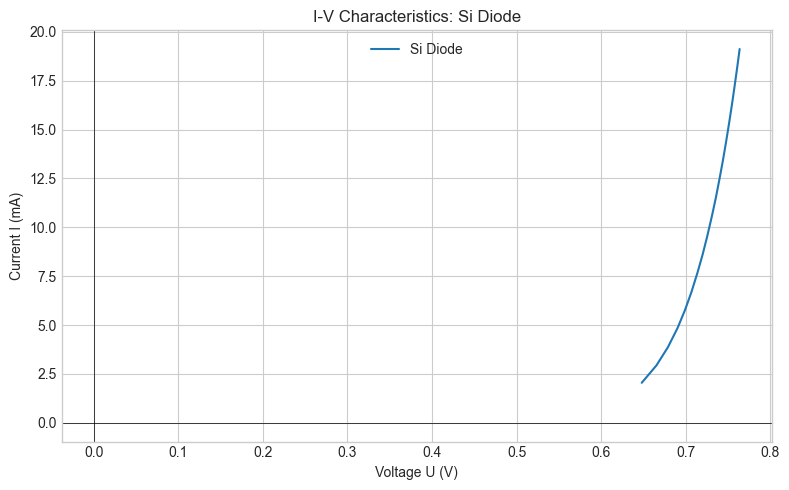
\includegraphics[width=0.45\linewidth]{../E14/Si.png}
  \caption{Forward $I$--$V$ characteristics of the silicon diode.}
  \label{fig:e14_iv_si}
\end{figure}

\begin{figure}[H]
  \centering
  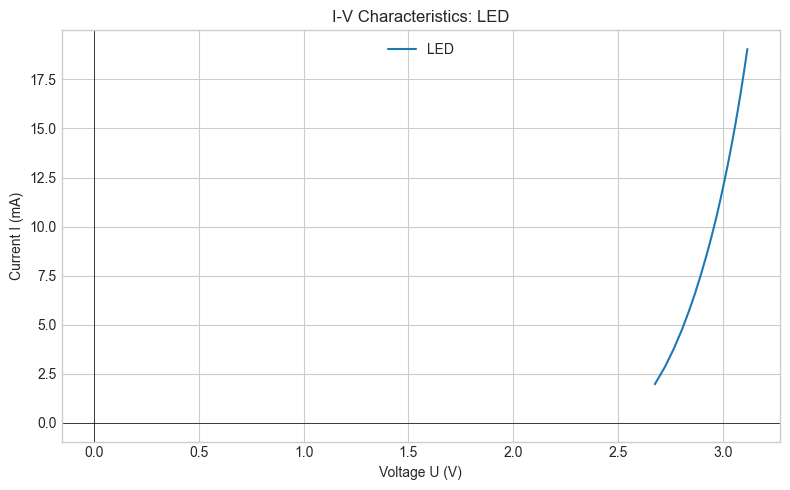
\includegraphics[width=0.45\linewidth]{../E14/LED.png}
  \caption{Forward $I$--$V$ characteristics of the LED.}
  \label{fig:e14_iv_led}
\end{figure}


% ─────────────────────────────────────────────────────────────────────────────
\section{E17e: Fourier Analysis of Coupled Electric Oscillations}
% ─────────────────────────────────────────────────────────────────────────────

\subsection{Method}

Two identical LC circuits were coupled in four configurations: capacitively
in the low-point arrangement, capacitively in the high-point arrangement,
through a single-circuit excitation that produces amplitude beats, and
inductively via variable coil separation. In each case, the free-oscillation
frequency spectrum was recorded via FFT on the PicoScope, and the in-phase
and out-of-phase eigenfrequencies $f_1$ and $f_2$ were extracted by peak
detection. The coupling coefficient follows from
\begin{equation}
  k = \frac{f_2^2 - f_1^2}{f_2^2 + f_1^2},
  \label{eq:coupling_coeff}
\end{equation}
with $k = C_K/(C+C_K)$ for the low-point configuration or
$k = C/(C+C_K)$ for the high-point configuration. These relations were
inverted to recover the bare capacitance $C$ for each coupling capacitor
$C_K$.

\subsection{Results}

In the low-point coupling measurements, $k$ decreased monotonically from
$0.90$ at $C_K = 22.2\,\uF$ to $0.00$ at $C_K = 555.5\,\uF$,
with the recovered bare capacitance remaining stable around
$195$ to $257\,\uF$ for all but the largest value of $C_K$.

In the high-point coupling measurements, $k$ increased monotonically from
approximately zero at $C_K = 22.2\,\uF$ to $0.68$ at
$C_K = 500\,\uF$, consistent with the opposite-sign dependence
expected from the high-point circuit topology. The recovered $C$ was stable
at roughly $213$ to $240\,\uF$ for $C_K \geq 111\,\uF$, but
diverged unphysically for the two smallest values of $C_K$, reaching
$2.7\times10^{6}\,\uF$ and $-5.8\times10^{5}\,\uF$
respectively, where $k \approx 0$ makes the relation
$C = (1-k)C_K/k$ numerically unstable.

In the beat measurement, a beat period of $T_S = 8.24\,\text{ms}$ was
extracted from the frequency splitting of the two normal modes when only
one circuit was excited. This splitting is visible directly as an
amplitude-modulated, decaying oscillation in the time-domain trace shown in
Figure~\ref{fig:e17_beat}.

For the inductive coupling measurements, spectra were recorded for eight
coil separations, but the coupling coefficient $k_L$ and the mutual
inductance $M$ were not computed in the excerpt provided.

\subsection{Assessment}

The low-point and high-point capacitive coupling results are physically
consistent with theory. In the low-point configuration, $k \to 0$ as
$C_K \to \infty$, while in the high-point configuration, $k \to 0$ as
$C_K \to 0$, both in the direction expected, and the recovered bare
capacitance $C$ remains approximately constant across the bulk of each
dataset, as required since $C$ is a fixed physical quantity independent of
$C_K$. The breakdown of the recovered $C$ at $k \approx 0$ in the
high-point measurement is an expected consequence of the $1/k$ singularity
in $C = (1-k)C_K/k$, and these points should simply be excluded from any
averaged estimate of $C$ rather than reported as numerical results. The
inductive-coupling analysis appears incomplete in the available material
and should be finished by computing $k_L = M/L$ and
$\Delta\omega \approx k_L\omega_0$ for each of the eight coil separations,
ideally fitted to the expected $M(d)$ falloff for coaxial coils in order to
extract an effective coil radius or moment.

\begin{figure}[H]
  \centering
  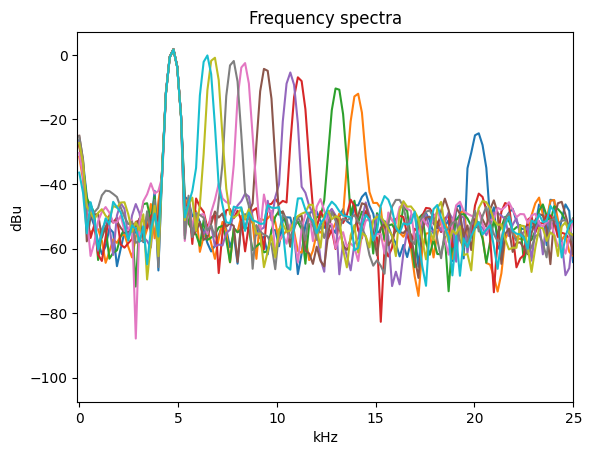
\includegraphics[width=0.45\linewidth]{../E17/frequency_spectra.png}
  \caption{Time-domain beat waveform for the high-point circuit with one
           branch excited, showing the characteristic amplitude envelope
           with period $T_S = 8.24\,\text{ms}$.}
  \label{fig:e17_beat}
\end{figure}

% ─────────────────────────────────────────────────────────────────────────────
\section{Overall Conclusion}
% ─────────────────────────────────────────────────────────────────────────────

Across all five experiments, fitted parameters generally agreed well with
component nominal values when the fitted feature had a sharp, well-localised
signature in the data. Examples include the RLC zero-crossing in E11e and
the diode forward threshold in E14e. Agreement was poorer in cases where
the measured response was broad, weakly constrained, or not adequately
described by the chosen model, as seen in the RL phase analysis of E11e,
the parallel-circuit fit of E12, the depletion-capacitance analysis of
E14e, and the transient measurements of E13He.

Despite these limitations, the experiments successfully demonstrated the
fundamental physical principles governing resonance, phase shifts,
transient response, semiconductor behaviour, and coupled oscillations.
Several extracted parameters agreed with theoretical expectations to within
one percent, confirming that nonlinear regression can provide highly
accurate parameter estimates when the underlying model adequately
represents the measured system.

The general lesson across this experiment series is that nonlinear
least-squares fits are only as reliable as the chosen fitting window and
the structural correctness of the model itself. Both should therefore be
checked against independent theoretical expectations before fitted
parameters are interpreted as physical quantities.

\printbibliography

\end{document}